\documentclass{../iot-lecture}

\subtitle{IoT Platforms}

\addbibresource{main.bib}

\begin{document}

\begin{frame}
  \titlepage{}
\end{frame}
\begin{frame}
  \frametitle{Outline}
  \tableofcontents{}
\end{frame}

\section{IoT Platforms, What \& Why?}

\begin{frame}
  \frametitle{Challenges\footfullcite{Rub2020}}
  \begin{itemize}
    \item Lack of a common data format and sharing standard.
    \begin{itemize}
      \item Two different sensors can monitor the same parameter using different unit of measurement.
    \end{itemize}
    \item Heterogeneity in networking and sensor technologies.
    \begin{itemize}
      \item Heterogeneous environment of IoT devices/plaforms that must be integrated into an interoperable one.
    \end{itemize}
  \end{itemize}
\end{frame}

\begin{frame}
  \frametitle{Challenges (Cont'd)}
  \begin{itemize}
    \item Lack of a standardized definition of environmental indicators.
    \begin{itemize}
      \item Standard doesn't consider clear metrics for water quality (i.e., temperature, pH, conductivity, and dissolved oxygen indicators)
    \end{itemize}
    \item Semantic interoperability between IoT solutions for the environment domain.
    \begin{itemize}
      \item Environmental studies can comprehend many phenomena through the observation/analysis of different features
        (i.e., earthquake can be predicted by vibrations or satellite image processing).
      \item A platform for environmental studies must model and explore the semantic relation between heterogeneous data sets.
    \end{itemize}
  \end{itemize}
\end{frame}

\begin{frame}
  \frametitle{Challenges (Cont'd)\footfullcite{Vresk2016}}
  \begin{itemize}
    \item Scalability
    \begin{itemize}
      \item The rapid development of technology enabled ubiquitous connectivity resuluting in a continues growth of a number of connected devices.
      \item In order to handle the growing amount of work, such as demand spikes, it is essential to implement scalability mechanisms and strategies that will maintain the system stability.
    \end{itemize}
  \end{itemize}
\end{frame}

\begin{frame}
  \frametitle{What is an IoT platform?}
  \begin{block}{Internet of Things Wiki\footfullcite{Top20IoTPlatforms}}
    In simple words the purpose of any \textbf{\color{YellowOrange} IoT device} is to connect with
    other IoT devices and applications (cloud-based mostly) to relay
    information using internet transfer protocols.

    The gap between the device sensors and data networks is filled
    by an \textit{\color{Green} IoT Platform}.
  \end{block}
\end{frame}

\begin{frame}
  \frametitle{What is their job?}
  \begin{itemize}
    \item Developers can develop their applications with ease
    \item End-users can see their dashboard and customize it
    \item The government can provide regulation on data
  \end{itemize}
\end{frame}

\begin{frame}
  \frametitle{Three-Layer IoT Architecture\footfullcite{Rub2020}}
  \begin{figure}
    \centering
    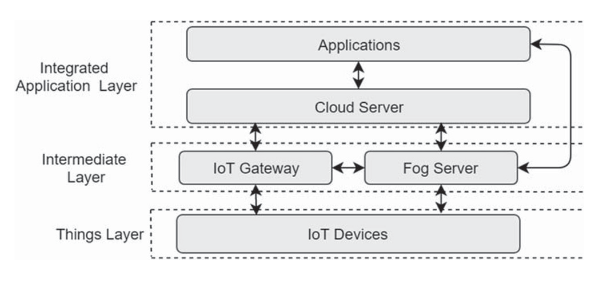
\includegraphics[width=\textwidth]{./img/three-layer-iot-architecture.png}
    \caption{structure of a three-layer IoT architecture}
  \end{figure}
\end{frame}

\begin{frame}
  \frametitle{Platforms' Components\footfullcite{Rub2020}}
  \begin{itemize}
    \item \textbf{\color{Cyan} Applications} process the gathered environment data, apply data mining and other big data
      techniques, train complex machine learning models, or keep monitoring the data to support decisions.
    \item \textbf{\color{YellowOrange} Cloud Server} provides the platform features required for data storage and processing to support
      the data used by applications.
    \item \textbf{\color{LimeGreen} IoT Gateway/Fog Server} primarily function as a data relay between IoT Devices and Cloud Server.
    \item \textbf{\color{RubineRed} IoT Devices} measure the environmental parameters and forward the measures to the gateway or fog server.
  \end{itemize}
\end{frame}

\begin{frame}
  \frametitle{Applications}
  \begin{itemize}
    \item Considered as clients that use the platform
    \item Can implement data mining techniques or near realtime monitoring
    \item \textit{Querying} the data from cloud and fog servers or receiving it in a \textit{publish/subscribe} approach.
  \end{itemize}
\end{frame}

\begin{frame}
  \frametitle{Cloud Server}
  \begin{itemize}
    \item Maintenance of the semantic model
    \item The storage and forwarding of data between gateways, fog servers and applications
    \item Protocols/Adapters component handles the adapters that implements the application layer protocols
  \end{itemize}
\end{frame}

\begin{frame}
  \frametitle{IoT Gateway}
  \begin{itemize}
    \item Protocols/Adapters component handles the adapters that implements the application layer protocols
    \item Verification of data integrity
    \item Processing of data to avoid the forwarding of meaningless messages
  \end{itemize}
\end{frame}

\begin{frame}
  \frametitle{Fog server}
  \begin{itemize}
    \item The Storage and Data Processing, the Publish/Subscribe Applications Services, and the Protocols/Adapters components have the
      same functionalities and implementation that the Cloud Server ones do.
  \end{itemize}
\end{frame}

\begin{frame}
  \frametitle{Scalability}
  \begin{itemize}
    \item There are two basic strategies for scaling:
    \begin{itemize}
      \item \textbf{\color{RubineRed} Vertical}: Adding additional resources to a single processing node.
      \item \textbf{\color{Cyan} Horizontal}: Adding more nodes to the overall system.
    \end{itemize}
    \item Opposite to vertical scaling, horizontal scaling represents a set of design practices and
      planned activities leading to an inherent distribution within the system.
  \end{itemize}
\end{frame}

\begin{frame}
  \frametitle{IoT Platform based on Microservices\footfullcite{Vresk2016}}
  \begin{itemize}
    \item To address the scalability and interoperability
    \item Define IoT concepts and platform based on orchestration of different IoT system components
    \item implemented in the form of microservices
  \end{itemize}
\end{frame}

\begin{frame}
  \frametitle{IoT Platform based on Microservices\footfullcite{Vresk2016} (Cont'd)}
  \begin{itemize}
    \item The \textsc{\color{YellowOrange} microservices} approach
    \begin{itemize}
      \item A relatively \textit{\color{LimeGreen} new term} in the software architecture pattern
      \item Present one of the solutions to the scalability problem in the IoT doamin
      \item Organizing distributed applications as a suite of services
      \item Each service is running in its own independent process context
        is designed to segregate one from service from another
    \end{itemize}
    \item Internal cross-service communication is implemented through proprietary interfaces
    \begin{itemize}
      \item relying on lightweight TCP/UDP-based application protocols.
    \end{itemize}
  \end{itemize}
\end{frame}

\begin{frame}
  \frametitle{IoT Platform based on Microservices\footfullcite{Vresk2016} (Cont'd)}
  \begin{itemize}
    \item Possibility to independently \textbf{\color{YellowOrange} deploy} and \textbf{\color{LimeGreen} scale} each service
    \begin{itemize}
      \item A service may be deployed as serveral instances
      \item Difference services may be hosted on the same server
      \item In monolithic architecture a small change in the application code requires the application/service
        to be completely rebuilt and redeployed.
      \item IoT relies on the integration of a large number of technologies, so monolithic based approach
        does not represent a suitable solution.
    \end{itemize}
  \end{itemize}
\end{frame}

\begin{frame}
  \frametitle{Communication Patterns\footfullcite{Vresk2016}}
  \begin{itemize}
    \item Telemetries
    \item Commands
    \item Queries
    \item Notifications
    \item Asynchronous and Synchronous Data Processing
  \end{itemize}
\end{frame}

\begin{frame}
  \frametitle{Traffic Patterns}
  \begin{itemize}
    \item Periodic
    \item Event Triggered
    \item Self Triggered
  \end{itemize}
\end{frame}

\begin{frame}
  \frametitle{Microservices Interactions\footfullcite{Vresk2016}}
  \begin{itemize}
    \item Interactions among different microservices are restricted to data exchange using only microservice-exposed interfaces.
  \end{itemize}
\end{frame}

\begin{frame}
  \frametitle{Data Model\footfullcite{Vresk2016}}
  \begin{itemize}
    \item Data are at the heart of every information system.
    \item Without connected devices being able to capture, transfer, analyse, report and act on data
    \begin{itemize}
      \item The benefits of the IoT would not be achievable
    \end{itemize}
    \item Applying \textit{\color{YellowOrange} semantic technology} promotes interoperability among resources, and facilitates data access, integration and knowledge extraction.
  \end{itemize}
\end{frame}

\begin{frame}
  \frametitle{Why a Reference Architecture\footfullcite{Guth2016}}
  \begin{itemize}
    \item Although IoT platforms provide similar or even equal functionality, their implementation and the underlying technologies differ.
    \item Diverse concepts and architectures, which complicates a comparison of multiple platforms.
    \item Users have to dive deep into the platforms' descriptions and have to understand each architecture and their components from scratch.
  \end{itemize}
\end{frame}

\begin{frame}
  \frametitle{Reference Architecture\footfullcite{Guth2016}}
  \begin{figure}
    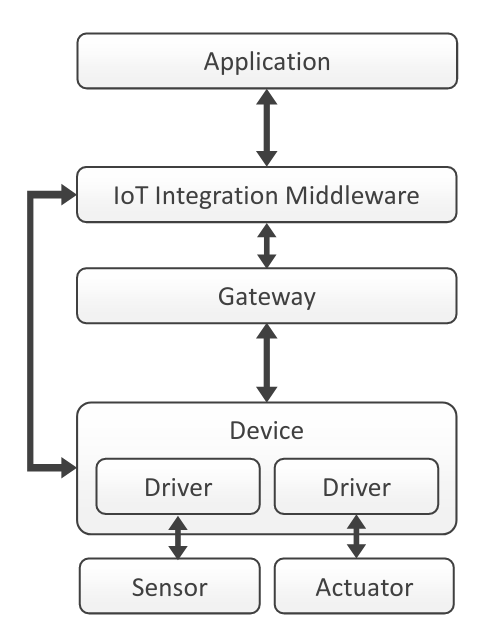
\includegraphics[height=.8\textheight]{./img/iot-ref-arch.png}
  \end{figure}
\end{frame}

\begin{frame}
  \frametitle{Sensor}
  \begin{itemize}
    \item A hardware component
    \item Measures parameters of its physical environment and translate them into electrical signals
    \item May be configured using \textit{software}
    \item Cannot run software itself
    \item \textit{\color{YellowOrange} Sensors} are connected to or are integrated into a \textit{\color{LimeGreen} Device} to which the gathered data is sent
  \end{itemize}
\end{frame}

\begin{frame}
  \frametitle{Actuator}
  \begin{itemize}
    \item A hardware component
    \item Act upon, control, or manipulate the physical environment
    \item Cannot run software itself
    \item \textit{\color{RubineRed} Actuators} receive commands from their connected \textit{\color{LimeGreen} Device}
  \end{itemize}
\end{frame}

\begin{frame}
  \frametitle{Device}
  \begin{itemize}
    \item A hardware component
    \item Connected to \textit{\color{RubineRed} Actuators} and/or \textit{\color{YellowOrange} Sensors} wires or wirelessly or even integrates these components.
    \item Process data from \textit{\color{YellowOrange} Sensors}
    \item Control \textit{\color{RubineRed} Actuators}
    \item Typically software in the form of \textbf{\color{Purple} Drivers} is required
    \item Devices are the entry point of the physical environment to the digital world
    \item Devices are:
    \begin{enumerate}
      \item Self-Contained and build a black box of functionality
      \item Connected to another system e.g.\ to an IoT Integration Middleware
    \end{enumerate}
  \end{itemize}
\end{frame}

\begin{frame}
  \frametitle{Gateway}
  \begin{itemize}
    \item Devices are connected to a \textit{\color{Cyan} Gateway} in cases when the \textit{\color{LimeGreen} Devices} is not capable of directly connecting to further systems.
    \begin{itemize}
      \item Communication forwarding
      \item Protocol translation
    \end{itemize}
    \item Gateways must support communication protocols and technologies in both direction
    \item May already execute some data processing functions such as data aggregation, depending on its processing capabilities.
  \end{itemize}
\end{frame}

\begin{frame}
  \frametitle{IoT Integration Middleware}
  \begin{itemize}
    \item Receiving data from the connected \textit{\color{LimeGreen} Devices}
    \item Process the received data
    \begin{itemize}
      \item Evaluating condition-action rules
      \item Provide the received data to connected Applications
      \item Control \textit{\color{LimeGreen} Devices} in terms of sending commands
    \end{itemize}
  \end{itemize}
\end{frame}

\begin{frame}
  \frametitle{Application}
  \begin{itemize}
    \item Represents software that uses the \textit{\color{TealBlue} IoT Integration Middleware} to gain insight into the physical environment
    \item Request \textit{\color{YellowOrange} Sensor} data
    \item Control physical actions using \textit{\color{RubineRed} Actuators}
  \end{itemize}
\end{frame}

\begin{frame}
  \frametitle{Related Works}
  \begin{itemize}
    \item Three-Layered Architecture
    \item Five-Layered Architecture
    \item Cisco Seven-Layered IoT Reference Model
  \end{itemize}
\end{frame}

\begin{frame}
  \frametitle{Big Picture}
  \begin{figure}
    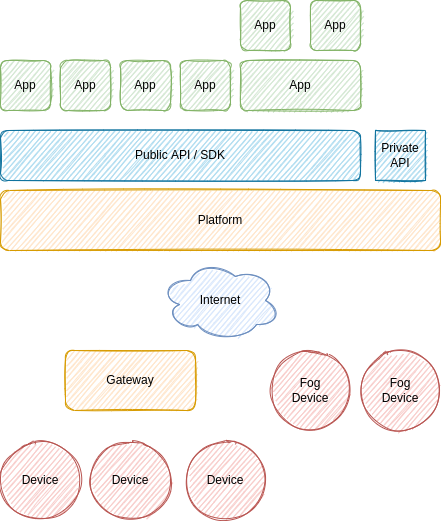
\includegraphics[height=.8\textheight]{./img/big-picture.png}
  \end{figure}
\end{frame}

\begin{frame}
  \frametitle{Platform}
  \begin{figure}
    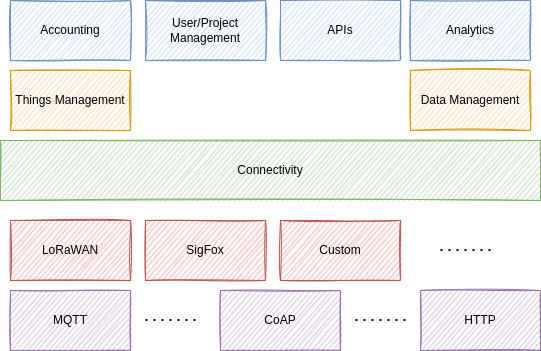
\includegraphics[width=\textwidth]{./img/platform.png}
  \end{figure}
\end{frame}

\section{Non Functional Requirements}

\begin{frame}
  \frametitle{Availability}
  \begin{itemize}
    \item Database Replication
    \item Handle Physical Machine/Network failures
    \item Handle Software Module failures
    \item \ldots
  \end{itemize}
\end{frame}

\begin{frame}
  \frametitle{Security}
  \begin{itemize}
    \item Using secure protocols e.g.\ HTTPS, MQTTS, \ldots
    \item JWT Authentication/Authorization
    \item Server Hardening
    \item \ldots
  \end{itemize}
\end{frame}

\begin{frame}
  \frametitle{Scalability}
  \begin{itemize}
    \item Large number of concurrent connected devices
    \item Different kind of protocols and connection methods
    \item \ldots
  \end{itemize}
\end{frame}

\section{Quality of Context}

\begin{frame}
  \frametitle{Introduction \footfullcite{Jagarlamudi2022}}
  \begin{itemize}
    \item Many IoT applications are becoming context-aware by obtaining seamless access to inferred IoT data
    \begin{itemize}
      \item Which is known as \textit{Context}
    \end{itemize}
  \end{itemize}
  \begin{block}{}
    \textit{Context} is any information that can be used to characterise the situation of an entity.
    An entity is a person, place, or object that is considered relevant to the interaction between a user and an application
    including the user and applications themselves.
  \end{block}
\end{frame}

\begin{frame}
  \frametitle{Introduction \footfullcite{Jagarlamudi2022} (Cont'd)}
  \begin{itemize}
    \item The context-aware IoT applications and the data sources are populary known as the:
    \begin{itemize}
      \item Context consumers (CCs)
      \item Context providers (CPs)
    \end{itemize}
    \item CCs attain seamless context access (access to desired context from the available CPs)
    \item \textit{\color{YellowOrange} through} context management platforms (or CMPS)
  \end{itemize}
\end{frame}

\begin{frame}
  \frametitle{Context Management Platform \footfullcite{Jagarlamudi2022} (Cont'd)}
  \begin{itemize}
    \item Mediates between the CPs and CCs
    \item Handles storage and processing tasks
    \begin{itemize}
      \item from gathering the CC's requirementes to delivering context back to it
    \end{itemize}
    \item Performs various interlinked processes, which are together known as the context lifecycle, for processing each request of a CC. These processes include:
    \begin{itemize}
      \item acquisition
      \item modelling
      \item reasoning
      \item dissemination
    \end{itemize}
    \begin{block}{}
      In \textit{context acquisition} CMP obtains the relevant raw data from CPs based on the CC's requirementes.
      Then, \textit{context modelling and reasoning} transform the low-level context into meaningful infromation.
      Finally, in \textit{context dissemination}, the CMP delivers high-level context to CCs.
    \end{block}
  \end{itemize}
\end{frame}

\section{SenML}

\begin{frame}
  \frametitle{Sensor Measurement List (SenML)}
  \begin{itemize}
    \item Format specification for representing simple sensor measurements and device parameters.
    \item Representations are defined in
    \begin{itemize}
      \item Javascript Object Notation (JSON)
      \item Concise Binary Object Representation (CBOR)
      \item Extensible Markup Language (XML)
      \item Efficient XML Interchange (EXI)
    \end{itemize}
  \end{itemize}
\end{frame}

\begin{frame}[fragile]
  \frametitle{SenML in Action}
  \begin{minted}[bgcolor=Black]{json}
[
  {
    "n":"urn:dev:ow:10e2073a01080063",
    "u": "Cel",
    "v": 23.1
  }
]
  \end{minted}
\end{frame}

\begin{frame}
  \frametitle{SenML in Action (Cont'd)}
  \begin{itemize}
    \item Temperature gauge encoded in the JSON syntax
    \item The array has a single SenML record
    \item sensor's name is \textit{``urn:dev:ow:10e2073a01080063''}
    \item sensor's value is \textit{23.1 degrees Celsius}
  \end{itemize}
\end{frame}

\section{OneM2M}

\begin{frame}
  \frametitle{Application Development Support with Mobius and \&Cube}
  \begin{figure}
    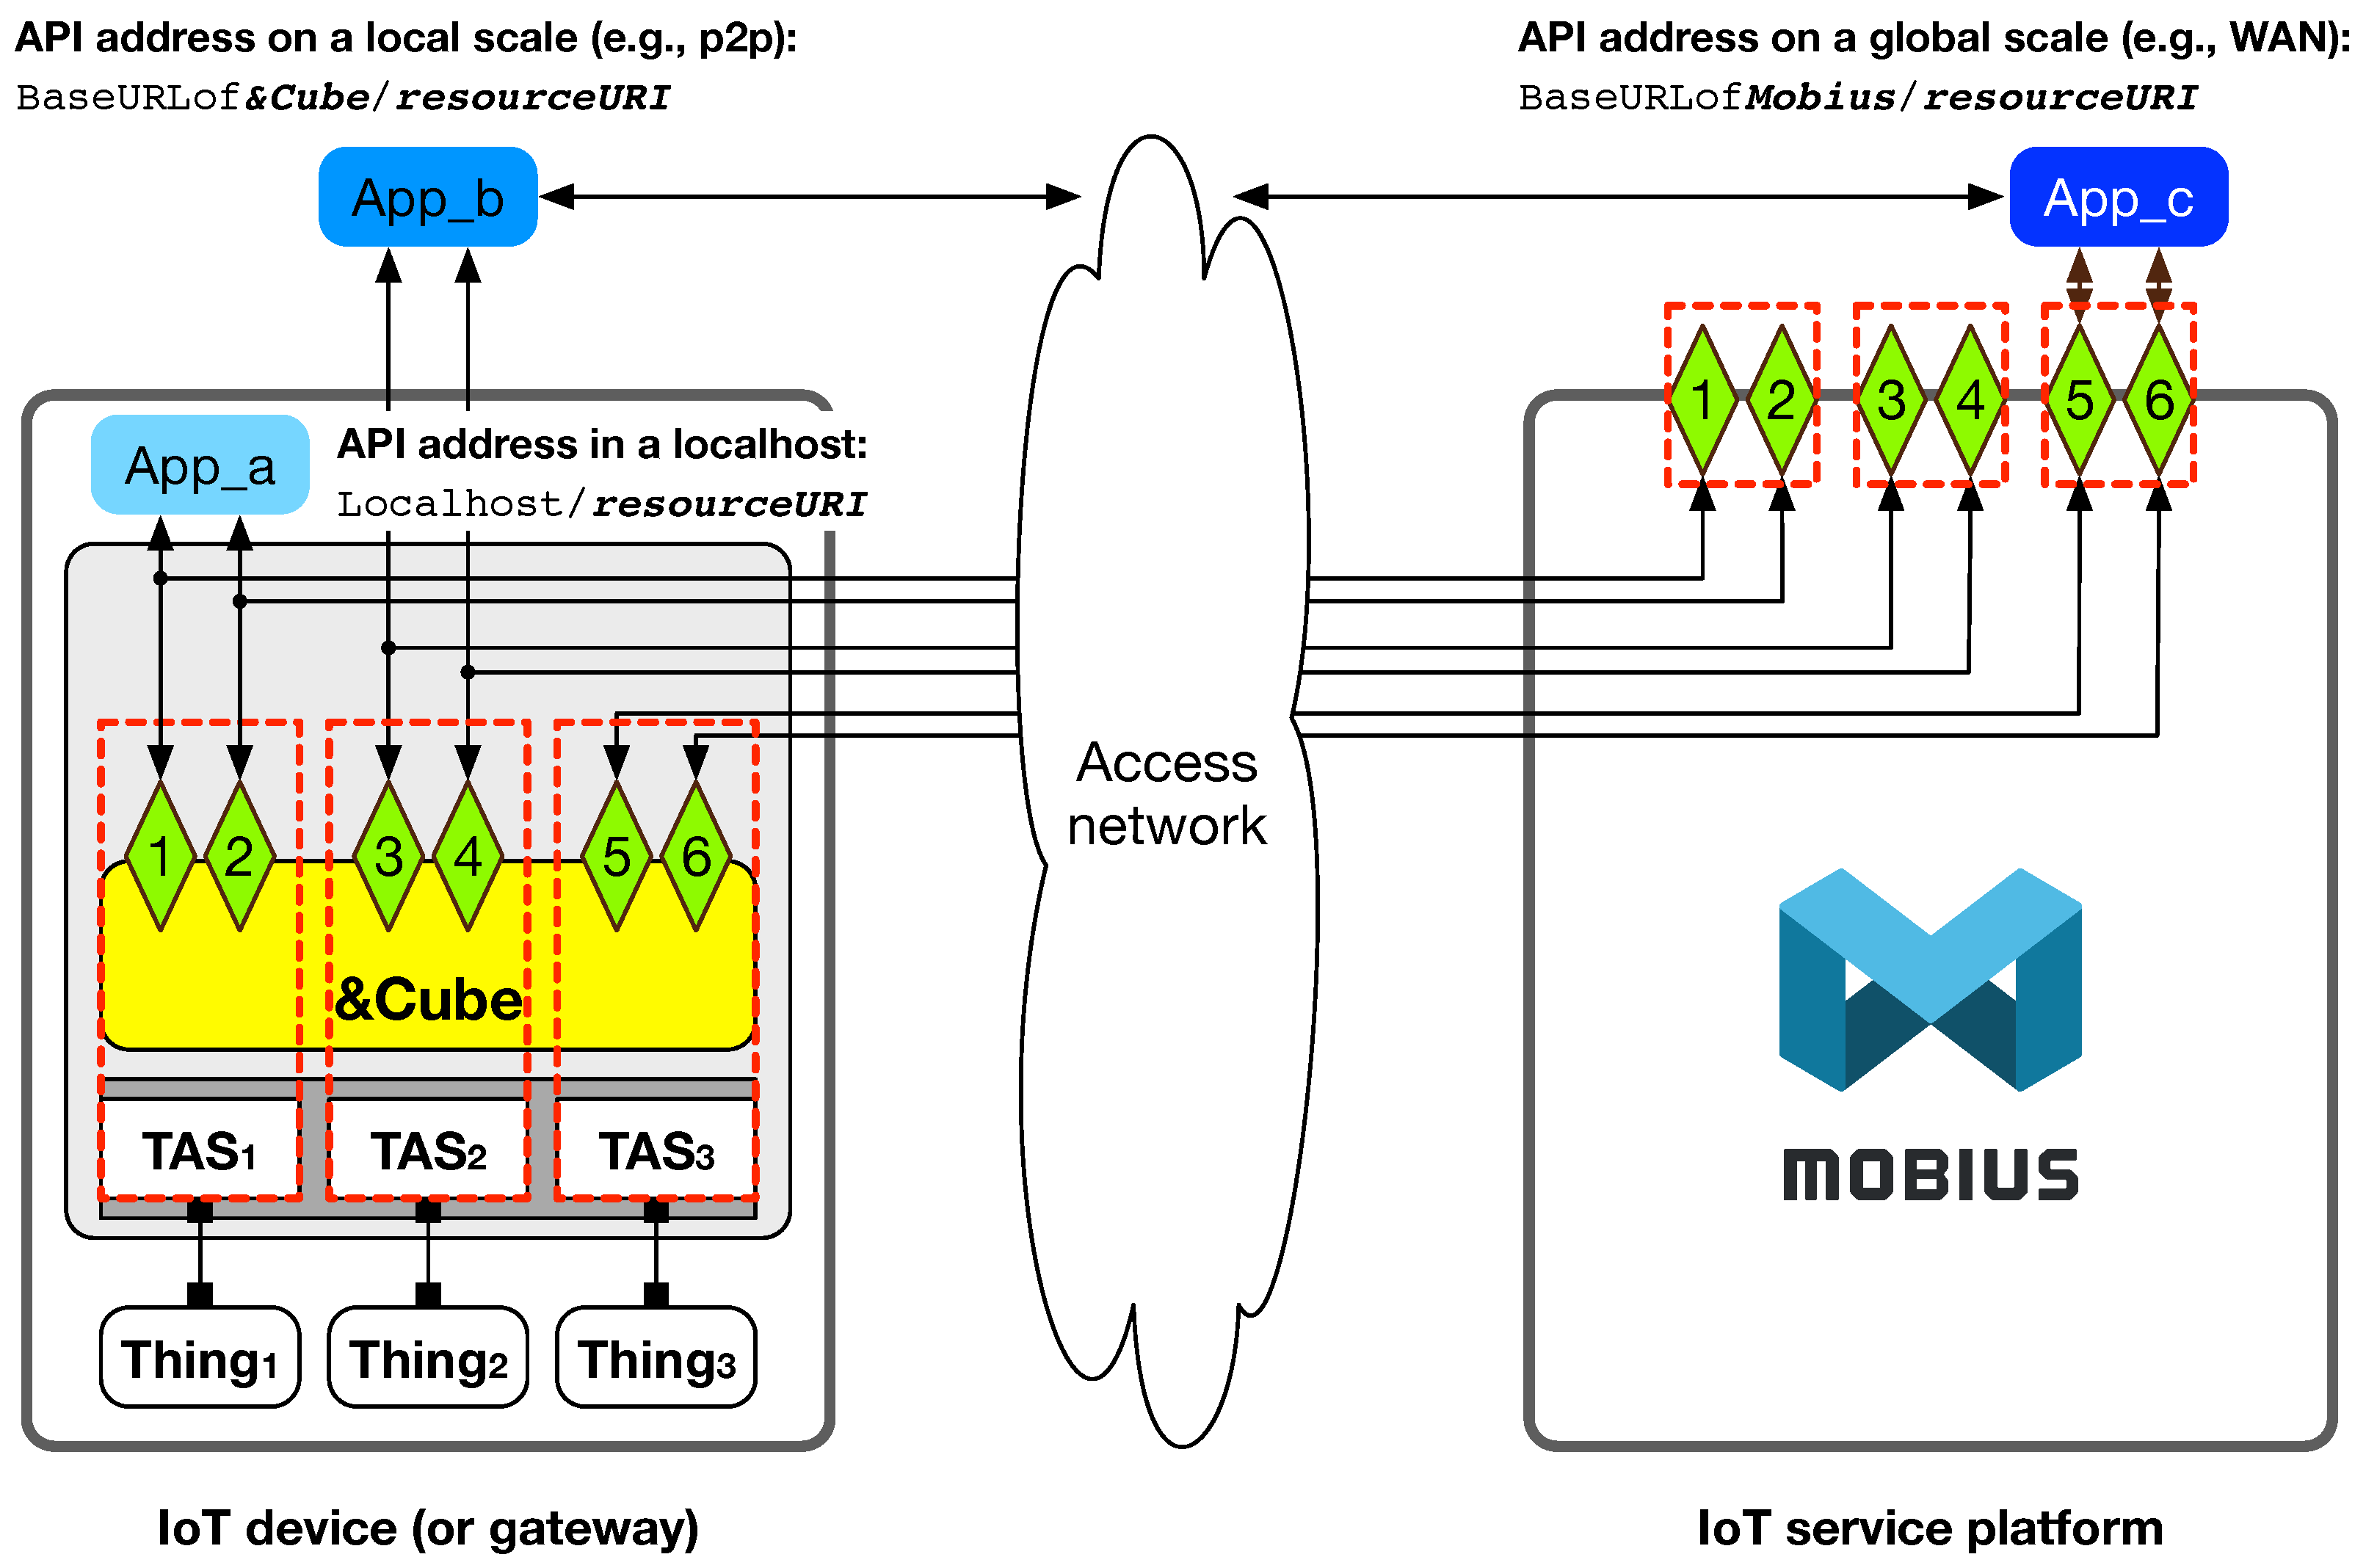
\includegraphics[width=\textwidth]{./img/mobius-amp-cube-app-dev-support.png}
    \caption{\scriptsize Application development support with Mobius and \&Cube on several scales\~\cite{Kim2016}}
  \end{figure}
\end{frame}

\section{OneDM}

%\begin{frame}[allowframebreaks]
%  \printbibliography%
%\end{frame}

\end{document}
